% Figure: two paths from an interactive prover to a first-order ATP (part 1).
% Build: pdflatex two_paths.tex  (run inside figures/)
\documentclass[tikz,border=6pt]{standalone}
\usetikzlibrary{arrows.meta}
\begin{document}
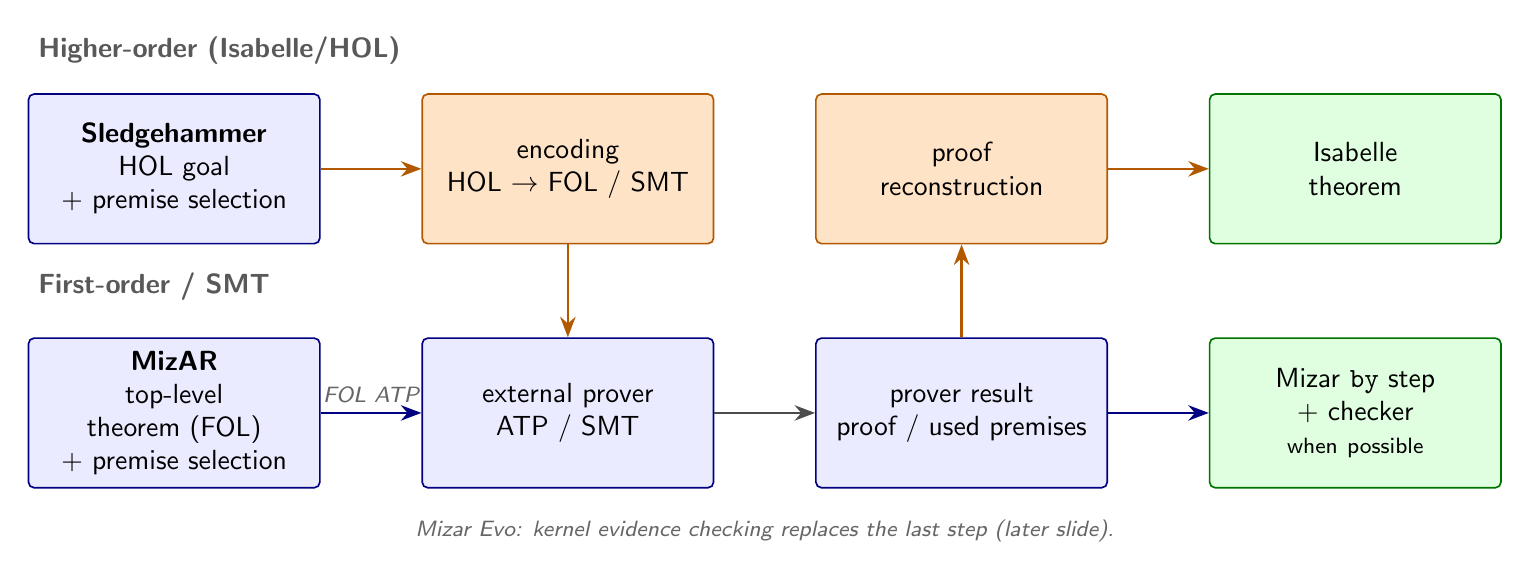
\begin{tikzpicture}[
  font=\sffamily,
  stepbox/.style={draw, rounded corners=2pt, align=center, text width=34mm,
               minimum height=19mm, inner sep=1.5mm, line width=0.6pt,
               fill=blue!8, draw=blue!50!black, font=\sffamily\normalsize},
  gap/.style={stepbox, fill=orange!22, draw=orange!70!black},
  check/.style={stepbox, fill=green!12, draw=green!45!black},
  head/.style={font=\sffamily\normalsize\bfseries, text=black!65, anchor=west},
  flow/.style={-{Stealth[length=2.6mm]}, line width=0.9pt, black!70},
  note/.style={font=\sffamily\footnotesize\itshape, text=black!60, align=center},
]
  % Higher-order input and output; proof search runs in the lower layer.
  \node[head] at (-18.5mm,15mm) {Higher-order (Isabelle/HOL)};
  \node[stepbox] (l1) at (0,0) {\textbf{Sledgehammer}\\ HOL goal\\ + premise selection};
  \node[gap] (l2) at (50mm,0) {encoding\\ HOL $\to$ FOL / SMT};
  \node[gap] (l5) at (100mm,0) {proof\\ reconstruction};
  \node[check] (l6) at (150mm,0) {Isabelle\\ theorem};
  \draw[flow, orange!70!black] (l1) -- (l2);
  \draw[flow, orange!70!black] (l5) -- (l6);

  % The central stages show a common interface, not a shared prover run.
  \node[head] at (-18.5mm,-15mm) {First-order / SMT};
  \node[stepbox] (r1) at (0,-31mm) {\textbf{MizAR}\\ top-level\\ theorem (FOL)\\ + premise selection};
  \node[stepbox] (r3) at (50mm,-31mm) {external prover\\ ATP / SMT};
  \node[stepbox] (r4) at (100mm,-31mm) {prover result\\ proof / used premises};
  \node[check] (r6) at (150mm,-31mm) {Mizar \texttt{by} step\\ + checker\\ \footnotesize when possible};
  \draw[flow, orange!70!black] (l2.south) -- (r3.north);
  \draw[flow] (r3) -- (r4);
  \draw[flow, orange!70!black] (r4.north) -- (l5.south);
  \draw[flow, blue!50!black] (r1) -- node[note, above] {FOL ATP} (r3);
  \draw[flow, blue!50!black] (r4) -- (r6);
  \node[note] at (75mm,-46mm)
    {Mizar Evo: kernel evidence checking replaces the last step (later slide).};
\end{tikzpicture}
\end{document}
